\section{User management}
\label{sec:USR_user_management}

Le app rivolte ad una comunità di utenti/clienti devono necessariamente implementare i meccanismi di gestione dell'utente.

I meccanismi di gestione utente base sono:
\begin{itemize}
\item login dell'utente
\item signup dell'utente
\item ogout dell'utente
\item gestione del profilo utente
\end{itemize}

A questi, possono essere associati meccanismi di gestione avanzati, quali:
\begin{itemize}
\item meccanismo di verifica email
\item meccanismo di cambio email
\item meccanismo di recovery/reset password
\item meccanismo di cambio password
\end{itemize}

I meccanismi di gestione avanzata, che prevedono l'uso della mail, devono necessariamente basarsi su un servizio di gestione della mail.
Sfida del presente progetto, è riuscire ad incapsulare tali meccanismi/comportamenti in relativi elementi, per permettere così di integrare la gestione dell'utente con la stessa semplicità con cui si inseriscono elementi HTML in una pagina.


\subsection{User Management services}
\label{subsec:USR_user_management_services}
In questa sezione si parla dei vari servizi esistenti per la gestione dell'utente come: Stormpat, Userapp e Auth0.

\subsubsection{Stormpath}

Stormpath is a User Management API that reduces development time with instant-on, scalable user infrastructure. Stormpath's intuitive API and expert support make it easy for developers to authenticate, manage and secure users and roles in any application.

At Stormpath, we have a simple goal: give developers a complete user management system, so you can focus on building great applications.\cite{usr_stormpath}

\begin{itemize}
\item Pre-built authentication \& authorization.
\item Schemaless, secure user data \& profiles.
\item Code-free Active Directory, Facebook \& Google login.
\item Open Source SDKs \& complete sample apps.
\end{itemize}

\begin {figure}[h]
\graphicspath{{images/chapter_USR/}}
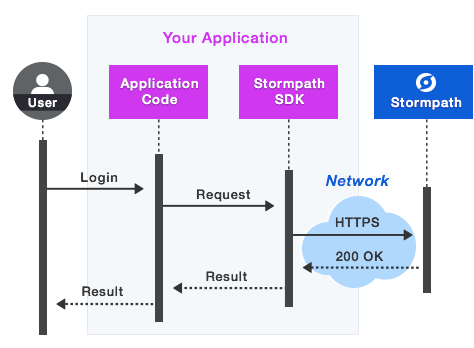
\includegraphics[width=\textwidth]{stormpath}
\caption{Stormpath User Management API}
\end {figure}

\subsubsection{Userapp}

UserApp is a cloud-based user management API for web apps. The purpose is to relieve developers from having to program logic for login, sign up, calculate payments, turn on or off features, etc. And instead focus on their core product.

UserApp provides you with user management functionality that results in faster development, faster revenue, more users, and the ability to serve your users better by engaging with them more efficiently.\cite{usr_userapp}

\begin{itemize}
\item User authentication - Have your user authentication ready today. You're just a few lines of code away with one of our SDKs.
\item One-click integrations - Integrate your users with third-party services with just one click.
\item Mobile, web, and server - No matter where you need to integrate your user authentication, we got you covered.
\end{itemize}

\subsubsection{Auth0}

Auth0 is an enterprise-grade platform for modern identity.
We give you tools that eliminate the friction of authentication for your applications and APIs - all accessible through your account dashboard.\cite{usr_auth0}

\begin {figure}[h]
\graphicspath{{images/chapter_USR/}}
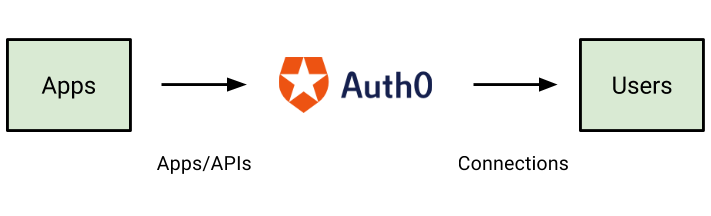
\includegraphics[width=\textwidth]{auth0}
\caption{Auth0 Overview}
\end {figure}

You can connect any application, written on any language or stack to Auth0, and separately define how users of that application authenticate:

\begin{itemize}
\item Custom credentials: username/passwords.
\item Social network logins: Google, Facebook, Twitter and any OAuth2 or OAuth1 provider.
\item Enterprise directories: LDAP, Google Apps, Office 365, ADFS, AD, SAML-P, WS-Federation, etc.,
\item Password-less systems: TouchID, one time codes on SMS.
\end{itemize}


\subsection{User Management API in StrongLoop LoopBack}

x-project is based on StrongLoop LoopBack on the server side.
LoopBack provides User Management.


Per la gestione della email, LoopBack si può connettere a vari providers.

Nello specifico, è stato implementata la connessione con il servizio di MailChimp chiamato Mandrill (vedi sezione...)
